\documentclass[12pt]{beamer}
\newenvironment{ConCodigo}[1]
  {\begin{frame}[fragile,environment=ConCodigo]{#1}}
  {\end{frame}}
\graphicspath{{Imagenes/}{../Imagenes/}}
\usepackage[utf8]{inputenc}
\usepackage[spanish]{babel}
\usepackage{hyperref}
\usepackage{etex}
%\reserveinserts{28}
\usepackage{amsmath}
\usepackage{amsthm}
\usepackage{mathtools}
\usepackage{multicol}
\usepackage{multirow}
\usepackage{tabulary}
\usepackage{booktabs}
\usepackage{nccmath}
\usepackage{physics}
\usepackage{biblatex}
\usepackage[outdir=./]{epstopdf}
%\epstopdfsetup{outdir=./}
\usepackage{graphicx}
%\usepackage{enumitem,xcolor}
\usepackage{siunitx}
%\sisetup{scientific-notation=true}
%\usepackage{fontspec}
\usepackage{lmodern}
\usepackage{float}
\usepackage[format=hang, font=footnotesize, labelformat=parens]{caption}
\usepackage[autostyle,spanish=mexican]{csquotes}
\usepackage{standalone}
\usepackage{blkarray}
\usepackage{algorithm}
\usepackage{algorithmic}
\usepackage{tikz}
\usepackage[siunitx, RPvoltages]{circuitikz}
\usetikzlibrary{arrows,patterns,shapes}
\usetikzlibrary{decorations.markings}
\usetikzlibrary{arrows}
\usepackage{color}
\usepackage{xcolor}
%\usepackage{beton}
%\usepackage{euler}
%\usepackage[T1]{fontenc}
\usepackage[sfdefault]{roboto}  %% Option 'sfdefault' only if the base font of the document is to be sans serif
\usepackage[T1]{fontenc}
\renewcommand*\familydefault{\sfdefault}
\DeclareGraphicsExtensions{.pdf,.png,.jpg}
\usepackage{hyperref}
\renewcommand {\arraystretch}{1.5}
\newcommand{\python}{\texttt{python}}
\usefonttheme[onlymath]{serif}
\setbeamertemplate{navigation symbols}{}
\usetikzlibrary{patterns}
\usetikzlibrary{decorations.markings}
\tikzstyle{every picture}+=[remember picture,baseline]
%\tikzstyle{every node}+=[inner sep=0pt,anchor=base,
%minimum width=2.2cm,align=center,text depth=.15ex,outer sep=1.5pt]
%\tikzstyle{every path}+=[thick, rounded corners]
\setbeamertemplate{caption}[numbered]
\newcommand{\ptm}{\fontfamily{ptm}\selectfont}
%Se usa la plantilla Warsaw modificada con spruce
\mode<presentation>
{
  \usetheme{Warsaw}
  \setbeamertemplate{headline}{}
  \useoutertheme{default}
  \usecolortheme{albatross}
  \setbeamercovered{invisible}
}
% \AtBeginSection[]
% {
% \begin{frame}<beamer>{Contenido}
% \normalfont\mdseries
% \tableofcontents[currentsection]
% \end{frame}
% }

%Se usa la plantilla Madrid modificada con beaver
\mode<presentation>
{
  \usetheme{Madrid}
  \setbeamertemplate{headline}{}
  %\useoutertheme{infolines}
  \usecolortheme{beaver}
  \setbeamercovered{invisible}
  

\setbeamertemplate{section in toc}[sections numbered]
\setbeamertemplate{subsection in toc}[subsections numbered]
\setbeamertemplate{subsection in toc}{\leavevmode\leftskip=3.2em\rlap{\hskip-2em\inserttocsectionnumber.\inserttocsubsectionnumber}\inserttocsubsection\par}
\setbeamercolor{section in toc}{fg=blue}
\setbeamercolor{subsection in toc}{fg=blue}
\setbeamerfont{subsection in toc}{size=\small}

\setbeamertemplate{navigation symbols}{}
\setbeamertemplate{caption}[numbered]

}

\input{../Preambulos/pre_codigo}
\makeatletter
\setbeamercolor{section in foot}{bg=green!30!cyan, fg=black!90!orange}
\setbeamercolor{subsection in foot}{bg=red!30!cyan, fg=red}
%\setbeamercolor{date in foot}{bg=orange!30!cyan, fg=red}
\setbeamertemplate{footline}
{
  \leavevmode%
  \hbox{%
  \begin{beamercolorbox}[wd=.333333\paperwidth,ht=2.25ex,dp=1ex,center]{section in foot}%
    \usebeamerfont{section in foot} \insertsection
  \end{beamercolorbox}}%
  \begin{beamercolorbox}[wd=.333333\paperwidth,ht=2.25ex,dp=1ex,center]{subsection in foot}%
    \usebeamerfont{subsection in foot}  \insertsubsection
  \end{beamercolorbox}%
  \begin{beamercolorbox}[wd=.333333\paperwidth,ht=2.25ex,dp=1ex,right]{date in head/foot}%
    \usebeamerfont{date in head/foot} \insertshortdate{} \hspace*{2em}
    \insertframenumber{} / \inserttotalframenumber \hspace*{2ex} 
  \end{beamercolorbox}}%
  \vskip0pt%
\makeatother
\title{Cuadraturas Gaussianas}
\subtitle{Tema 2 - Operaciones matemáticas básicas}
\author{M. en C. Gustavo Contreras Mayén}
\date{22 de abril de 2020}
\institute{Facultad de Ciencias - UNAM}
\titlegraphic{\includegraphics[width=1.75cm]{Imagenes/escudo-facultad-ciencias}\hspace*{4.75cm}~%
   \includegraphics[width=1.75cm]{Imagenes/escudo-unam}
}
\newtheorem{miteorema}{Teorema}
\begin{document}
\maketitle
\fontsize{14}{14}\selectfont
\spanishdecimal{.}
\setbeamercolor{frametitle}{bg=blue!30!white}
\section*{Contenido}
\frame{\tableofcontents[currentsection, hideallsubsections]}
\section{Introducción}
\frame{\tableofcontents[currentsection, hideothersubsections]}
\subsection{Segunda parte de las cuadraturas}
\begin{frame}
\frametitle{Introducción}
Las fórmulas de Newton-Cotes implican, según la construcción, que los puntos de integración \emph{estén  igualmente espaciados}.
\\
\bigskip
Para un orden dado de la fórmula, los puntos $x_{i}$ y los pesos se seguirán directamente del polinomio de interpolación de Lagrange basado en los $n$ puntos de integración.
\end{frame}
\begin{frame}
\frametitle{Introducción}
En comparación, la idea básica de las llamadas \textoazul{cuadraturas gaussianas} consiste en \emph{elegir de manera óptima tanto los puntos (abscisas) como los pesos}, para lograr la máxima precisión para ciertas clases de integrandos (por ejemplo, polinomios).
interpolación de Lagrange basado en los $n$ puntos de integración.
\end{frame}
\begin{frame}
\frametitle{Introducción}
Al disponer de un número doble de parámetros ajustables (por separado, abscisas y pesos), se pueden construir, en principio, fórmulas de cuadratura de doble orden en comparación con las fórmulas de Newton-Cotes con el mismo número de puntos de integración.
\end{frame}
\section{Cuadraturas Gaussianas}
\frame{\tableofcontents[currentsection, hideothersubsections]}
\subsection{Definición de cuadraturas}
\begin{frame}
\frametitle{Cuadraturas Gaussianas}
Hemos visto que las fórmulas de Newton-Cotes para aproximar la intregral
\begin{align*}
\int_{a}^{b} f(x) \dd{x}
\end{align*}
trabajan muy bien si $f(x)$ es una función suave, como los polinomios.
\end{frame}
\begin{frame}
\frametitle{Cuadraturas Gaussianas}
También aplica para las cuadraturas Gaussianas, ya que son buenas para estimar integrales de la forma:
\begin{align*}
\int_{a}^{b} w(x) \, f(x) \dd{x}
\end{align*}
donde $w(x)$ se denomina \emph{función de peso} que puede contener singularidades, siempre y cuando sean integrables.
\end{frame}
\begin{frame}
\frametitle{Cuadraturas Gaussianas}
Un ejemplo de este tipo, sería la integral:
\begin{align*}
\int_{0}^{1} \left(1 + x^{2} \right) \, \ln x  \dd{x}
\end{align*}
\\
\bigskip
\pause
o cuando tenemos límites de integración infinitos
\begin{align*}
\int_{0}^{\infty} \exp(-x) \, \sin x \dd{x}
\end{align*}
éstos se pueden reacomodar para calcular la integral.
\end{frame}
\begin{frame}
\frametitle{Fórmulas de integración Gaussianas}
Las fórmulas de integración Gaussianas tiene la misma forma de las reglas de Newton-Cotes:
\begin{align*}
I = \sum_{i=0}^{n} A_{i} \, f(x_{i})
\end{align*}
donde $I$ representa la aproximación al valor de la integral, la diferencia radica en la forma en que se determinan los pesos $A_{i}$ y abscisas nodales $x_{i}$.
\end{frame}
\begin{frame}
\frametitle{Fórmulas de integración Gaussianas}
En la integración de Newton-Cotes los nodos se espacian uniformemente en $(a, b)$, es decir, estaban ya predeterminadas sus ubicaciones.
\\
\bigskip
En la cuadratura de Gauss, se eligen los nodos y los pesos de modo que con la ecuación para $I$, se obtiene la integral exacta si $f(x)$ es un polinomio de grado $2 \, n + 1$ o menor, es decir:
\end{frame}
\begin{frame}
\frametitle{Cuadratura Gaussiana}
\begin{align*}
\int_{a}^{b} w(x) \, P_{m}(x) \dd{x} = \sum_{i=0}^{n} A_{i} \, P_{m}(x_{i}), \hspace{1cm} m \leq 2 \, n + 1
\end{align*}
\pause
Una manera de determinar los pesos y las abscisas es sustituir 
\begin{align*}
P_{0}(x) &= 1 \\
P_{1}(x) &= x \\
\vdots \\
P_{2 \, n + 1}(x) &= x^{2 \, n + 1}
\end{align*}
\end{frame}
\begin{frame}
\frametitle{Cuadratura Gaussiana}
Es sustituir en la ecuación anterior y resolver el sistema de $2 \, n + 2$ ecuaciones:
\begin{align*}
\int_{a}^{b} w(x) \, x^{j} \dd{x} = \sum_{i=0}^{n} A_{i} \, x_{i}^{j}, \hspace{0.6cm} j = 0, 1, \ldots, 2 \, n + 1
\end{align*}
para las incógnitas $A_{i}$ y $x_{i}$.
\end{frame}
\begin{frame}
\frametitle{Ejemplo de una cuadratura Gaussiana}
Como ejemplo veamos: sea la función de peso $w(x)$, los intervalos de integración $a$, $b$ y $n$, tal que:
\begin{align*}
w(x)= \exp(-x) \hspace{0.5cm} a = 0, b = \infty, \hspace{0.3cm} n = 1
\end{align*}
\end{frame}
\begin{frame}[fragile]
\frametitle{Ejemplo de una cuadratura Gaussiana}
Las cuatro ecuaciones que determinan $x_{0}$, $x_{1}$, $A_{0}$ y $A_{1}$ son:
\begin{align*}
\int_{0}^{\infty} \exp(-x) \dd{x} &= A_{0} + A_{1} \\[0.5em]
\visible<2->{\int_{0}^{\infty} \exp(-x) \, x \dd{x} &= A_{0} \, x_{0} + A_{1} \, x_{1}} \\[0.5em]
\visible<3->{\int_{0}^{\infty} \exp(-x) \, x^{2} \dd{x} &= A_{0} \, x_{0}^{2}+ A_{1} \, x_{1}^{2}} \\[0.5em]
\visible<4->{\int_{0}^{\infty} \exp(-x) \, x^{3} \dd{x} &= A_{0} \, x_{0}^{3} + A_{1} \, x_{1}^{3}}
\end{align*}
\end{frame}
\begin{frame}
\frametitle{Ejemplo de una cuadratura Gaussiana}
Evaluando las integrales, obtenemos
\begin{align*}
A_{0} + A_{1} &= 1 \\[0.5em]
A_{0} x_{0} + A_{1} x_{1} &= 1 \\[0.5em]
A_{0} x_{0}^{2} + A_{1} x_{1}^{2} &= 2 \\[0.5em]
A_{0} x_{0}^{3} + A_{1} x_{1}^{3} &= 6
\end{align*}
\end{frame}
\begin{frame}
\frametitle{Ejemplo de una cuadratura Gaussiana}
Cuya solución es:
\begin{align*}
x_{0} &= 2 - \sqrt{2} \hspace{0.75cm} A_{0} = \dfrac{\sqrt{2} + 1}{2 \, \sqrt{2}} \\[0.5em]
x_{1} &= 2 + \sqrt{2} \hspace{0.75cm} A_{1} = \dfrac{\sqrt{2} - 1}{2 \, \sqrt{2}}
\end{align*}
\end{frame}
\begin{frame}
\frametitle{Ejemplo de una cuadratura Gaussiana}
Por tanto la fórmula de integración obtenida es:
\begin{align*}
\int_{0}^{\infty} \exp(-x) \, f(x) \dd{x} & \simeq \dfrac{1}{2 \, \sqrt{2}} \left[ \left( \sqrt{2} + 1 \right) \, f \left(2 - \sqrt{2} \right) + \right. \\[0.5em] 
&+ \left. \left( \sqrt{2} - 1 \right) \, f \left(2 + \sqrt{2} \right) \right]
\end{align*}
\pause
Debido a la no linealidad de las ecuaciones, este enfoque no va a funcionar bien para valores grandes de $n$.
\end{frame}
\begin{frame}
\frametitle{Métodos prácticos para la cuadratura}
Hay métodos prácticos para calcular $x_{i}$ y $A_{i}$ que requieren un cierto conocimiento de los polinomios ortogonales y su relación con la cuadratura de Gauss.
\\
\bigskip
Sin embargo, existen varias fórmulas \enquote{clásicas} de integración Gaussianas para los cuales, las abscisas y pesos han sido calculados y tabulados con gran precisión.
\end{frame}
\begin{frame}
\frametitle{Métodos prácticos para la cuadratura}
Estas fórmulas se pueden utilizar sin conocer la teoría detrás de ellas (en el semestre anterior, es decir el sexto de la carrera de Física, llevaste el curso de Matemáticas Avanzadas de la Física, por lo que ya tendrás conocimiento de estas funciones), ya que todo lo que uno necesita para la integración de Gauss son los valores de $x_{i}$ y $A_{i}$.
\end{frame}
\subsection{Polinomios ortogonales}
\begin{frame}
\frametitle{Polinomios ortogonales}
Los polinomios ortogonales se utilizan en muchas áreas de la física, de la matemática y del análisis numérico; se han estudiado a fondo y muchas de sus propiedades ya son conocidas. 
\end{frame}
\begin{frame}
\frametitle{Polinomios ortogonales}
Los polinomios $\varphi_{n}(x)$, con $n = 0, 1, 2,\ldots$ ($n$ es el grado del polinomio) se dice que forman un conjunto ortogonal en el intervalo $(a, b)$ con respecto a la función de peso $w(x)$ si
\begin{align*}
\int_{a}^{b} w(x) \, \varphi_{m}(x) \, \varphi_{n}(x) \dd{x} = 0, \hspace{0.5cm} m \neq n 
\end{align*}
\end{frame}
\begin{frame}
    \frametitle{Polinomios ortogonales}
El conjunto ortogonal se determina (con excepción de un factor constante) por: la elección de la función de peso y los límites de integración.
\\
\bigskip
Es decir, cada conjunto de polinomios ortogonales se asocia con ciertas funciones $w(x)$, y ciertos límites de integración: $a$ y $b$. El factor constante se especifica de manera estandarizada.
\end{frame}
\begin{frame}
\frametitle{Polinomios ortogonales}
A continuación se enlistan algunos de los polinomios ortogonales clásicos, la última columna indica la estandarización usada.
\end{frame}
\begin{frame}
\frametitle{Polinomios ortogonales}
\fontsize{12}{12}\selectfont
\begin{tabular}{| l | c | c | c | c | c |}
\hline
Nombre & Símbolo & $a$ & $b$ & $w(x)$ & $\int_{a}^{b} \left[ \varphi_{n} (x)\right]^{2} \dd{x} $ \\ \hline
Legendre & $p_{n}(x)$ & $-1$ & $1$ & $1$ & $2/(2n+1)$ \\
Chebyshev & $T_{n}(x)$ & $-1$ & $1$ & $(1 - x^{2})^{-1/2}$ & $\pi/2 \hspace{0.2cm} (n>0)$ \\
Laguerre & $L_{n}(x)$ & $0$ & $\infty$ & $e^{-x}$ & $1$ \\
Hermite & $H_{n}(x)$ & $-\infty$ & $\infty$ & $e^{x^{2}}$ & $\sqrt{\pi} \, 2^{n} \, n!$ \\ \hline
\end{tabular}
\end{frame}
\subsection*{Propiedades de los polinomios ortogonales}
\begin{frame}
\frametitle{Propiedades de los polinomios ortogonales}
Los polinomios ortogonales cumplen relaciones de recurrencia de la forma
\begin{align*}
a_{n} \, \varphi_{n+1} (x) = (b_{n} + c_{n} \, x) \varphi_{n} (x) - d_{n} \, \varphi_{n-1} (x)
\end{align*}
Si los dos primeros polinomios del conjunto se conocen, los otros elementos del conjunto pueden calcularse de la ecuación anterior. 
\end{frame}
\begin{frame}
\frametitle{Propiedades de los polinomios ortogonales}
Los coeficientes en la fórmula de recurrencia, junto con $\varphi_{0}(x)$ y $\varphi_{1}(x)$ son:
\fontsize{12}{12}\selectfont
\begin{tabular}{| l | c | c | c | c | c | c |}
\hline
Nombre & $\varphi_{0}(x)$ & $\varphi_{1}(x)$ & $a_{n}$ & $b_{n}$ & $c_{n}$ & $d_{n}$ \\ \hline
Legendre & $1$ & $x$ & $n+1$ & $0$ & $2\, n + 1$ & n \\
Chebyshev & $1$ & $x$ & $1$ & $0$ & $2$ & $1$ \\
Laguerre & $1$ & $1 - x$ & $n + 1$ & $2 \, n + 1$ & $-1$ & $n$ \\
Hermite & $1$ & $2 \, x$ & $1$ & $0$ & $2$ & $2$ \\ \hline
\end{tabular}
\end{frame}
\begin{frame}
\frametitle{Otra manera para obtener los polinomios}
Los polinomios ortogonales clásicos también se pueden obtener de las fórmulas:
\begin{align*}
P_{n}(x) &= \dfrac{(-1)^{n}}{2^{n}n!} \dv[n]{x} \left[ \left( 1 - x^{2} \right)^{n} \right] \\[0.5em]
T_{n}(x) &= \cos(n \, \cos^{-1} \, x), \hspace{0.3cm} n > 0 \\[0.5cm]
L_{n}(x) &= \dfrac{e^{x}}{n!} \dv[n]{x} \left( x^{n} \, e^{-x} \right) \\[0.5cm]
H_{n}(x) &= (-1)^{n} \, e^{x^{2}} \dv[n]{x} \left(e^{x^{2}} \right)
\end{align*}
\end{frame}
\begin{frame}
\frametitle{Derivadas de los polinomios ortogonales}
Las derivadas de los polinomios anteriores se pueden calcular de:
\begin{align*}
(1-x^{2}) \, P^{\prime}_{n}(x) &= n \, [-x \, P_{n}(x) + P_{n-1}(x) ] \\[0.5em]
(1-x^{2}) \, T^{\prime}_{n}(x) &= n \, [-x \, T_{n}(x) + n \, T{n-1}(x) ] \\[0.5em]
x \, L^{\prime}_{n} (x) &= n \, [ L_{n}(x) - L_{n-1}(x) ] \\[0.5em]
H^{\prime}_{n}(x) &= 2 \, n \, H_{n-1}(x)
\end{align*}
\end{frame}
\begin{frame}
\frametitle{Propiedades de los polinomios}
Algunas propiedades los polinomios ortogonales que son relevantes para la preceso de integración Gaussiana son:
\setbeamercolor{item projected}{bg=blue!70!black,fg=yellow}
\setbeamertemplate{enumerate items}[circle]
\begin{enumerate}[<+->]
\item $\varphi(x)$ tiene $n$ distintos ceros en el intervalo $(a, b)$
\item Los ceros de $\varphi_{n}(x)$ están entre los ceros de $\varphi_{n+1}(x)$
\seti
\end{enumerate}
\end{frame}
\begin{frame}
\frametitle{Propiedades de los polinomios}
\setbeamercolor{item projected}{bg=blue!70!black,fg=yellow}
\setbeamertemplate{enumerate items}[circle]
\begin{enumerate}
\conti
\item Cualquier polinomio $P_{n}(x)$ de grado $n$ puede expresarse de la forma:
\begin{align*}
P_{n}(x) =  \sum_{i=0}^{n} c_{i} \varphi_{i} (x)
\end{align*}
\item Se deduce de la ecuación anterior y de la propiedad de ortogonalidad que:
\begin{align*}
\int_{a}^{b} w(x) \, P_{n}(x) \varphi_{n + m} (x) \dd{x} = 0, \hspace{0.4cm} m \geq 0
\end{align*}
\end{enumerate}
\end{frame}
\subsection{Deduciendo las abscisas nodales y los pesos}
\begin{frame}
\frametitle{Deduciendo las abscisas nodales y los pesos}
Hay dos teoremas importantes que son de gran utilidad para apoyarnos y tomar sus resultados para la integración Gaussiana, la demostración es relativamente sencilla, pero no los demostraremos aquí, puede ser un buen ejercicio fuera de clase.
\end{frame}
\begin{frame}
\frametitle{Teorema 1}
\begin{miteorema}
Las abscisas nodales $x_{0}, x_{1}, \ldots, x_{n}$ son los ceros del polinomio $\varphi_{n+1}(x)$  que pertenece al conjunto ortogonal definido por
\begin{align*}
\int_{a}^{b} w(x) \, \varphi_{m}(x) \, \varphi_{n}(x) \dd{x} = 0, \hspace{0.5cm} m \neq n
\end{align*}
\end{miteorema}
\end{frame}
\begin{frame}
\frametitle{Teorema 2}
\begin{miteorema}
\begin{align*}
A_{i} = \int_{a}^{b} w(x) \, \mathcal{L}_{i} (x) \dd{x}, \hspace{1cm} i = 0, 1, \ldots, n
\end{align*}
donde $\mathcal{L}_{i} (x)$ son las funciones cardinales de Lagrange que abarcan los nodos $x_{0}, x_{1}, \ldots, x_{n}$.
\end{miteorema}
\end{frame}
\begin{frame}
\frametitle{Deduciendo las abscisas nodales y los pesos}
No es difícil calcular los ceros $x_{i}$, $i = 0, 1, \ldots, n$ de un polinomio $\varphi_{n+1} (x)$ que pertenece a un conjunto ortogonal, podemos usar alguno de los métodos discutidos en la parte de cálculo de raíces.
\\
\bigskip
Una vez conocidos los ceros, los pesos $A_{i}$, $i = 0, 1, \ldots, n$ pueden calcularse de la ecuación anterior.
\end{frame}
\begin{frame}
\frametitle{Fórmulas para calcular los pesos}
Se puede demostrar que los pesos se pueden calcular a partir de:
\begin{align*}
\mbox{Gauss-Legendre   }  A_{i} &= \dfrac{2}{(1-x^{2}_{i}) \, \left[P^{\prime}_{n+1} (x_{i}) \right]^{2}} \\[0.5em]
\mbox{Gauss-Laguerre   } A_{i} &= \dfrac{1}{x_{i} \, \left[L^{\prime}_{n+1} (x_{i}) \right]^{2}} \\[0.5em]
\mbox{Gauss-Hermite   } A_{i} &= \dfrac{2^{n+2} \, (n+1)! \, \sqrt{\pi}}{\left[ H^{\prime}_{n+1} (x_{i}) \right]^{2}}
\end{align*}
\end{frame}
\begin{frame}
\frametitle{Algunas abscisas y pesos}
Vamos a mencionar la expresión para algunas fórmulas de integración por cuadraturas gaussianas.
\\
\bigskip
La tabla de abscisas y pesos que se presenta a continuación, cubre para $n=1$ a $5$, y se redondea a seis decimales.
\end{frame}
\begin{frame}
\frametitle{Algunas abscisas y pesos}
Las operaciones con estos valores, se considera que funcionan bien si se hacen las cuentas a mano, en caso de requerir una mayor precisión o incluir un número  mayor de nodos, será necesario usar la computadora, siendo necesario consultar otras referencias\footnote{Abramowitz, M. y Stegun, I.A, Handbook of Mathematical Functions, Dover Publications, 1965.}.
\end{frame}
\subsection{Error en la cuadratura gaussiana}
\begin{frame}
\frametitle{Error en la cuadratura gaussiana}
El error $E$ en la cuadratura gaussiana debido al truncamiento
\begin{align*}
E = \int_{a}^{b} w(x) \, f(x) \dd{x}  - \sum_{i=0}^{n} A_{i} \, f(x_{i})
\end{align*}
es de la forma $E= K(n) f^{2 \,n + 2} (c) $, donde $a < c < b$, el valor de $c$ no se conoce, solamente los extremos.
\end{frame}
\begin{frame}
\frametitle{Error en la cuadratura gaussiana}
La expresión para $K(n)$ depende de la cuadratura en particular que se esté utilizando.
\\
\bigskip
Si las derivadas de $f(x)$ se pueden evaluar, el error de las fórmulas es útil para estimar el error en el intervalo.
\end{frame}
\subsection{Cuadratura Gauss-Legendre}
\begin{frame}[plain]
\frametitle{Cuadratura de Gauss-Legendre}
La fórmula para la cuadratura Gauss-Legendre es la siguiente:
\begin{align*}
\int_{-1}^{1} f(\xi) \dd{\xi} \approx \sum_{i=0}^{n} A_{i} \, f(\xi_{i})
\end{align*}
Los pesos y las abscisas nodales se presentan en la siguiente tabla:
\end{frame}
\begin{frame}
\frametitle{Pesos y abscisas}
\fontsize{10}{10}\selectfont
\begin{center}
\begin{tabular}{|c c c | c c c|}
\hline
$\pm \xi_{i}$ & & $A_{i}$ & $\pm \xi_{i}$ &  & $A_{i}$ \\ \hline
 & $n=1$ & & & $n=4$ & \\ %\hline
$0.577350$ & & $1.000000$ & $0.000000$ & & $0.568889$ \\ %\hline
 & $n=2$ & & $0.538469$ & & $0.478629$ \\ %\hline
$0.000000$ & & $0.888889$ & $0.906180$ & & $0.236927$ \\ %\hline
$0.774597$ & & $0.555556$ & & $n=5$ & \\ %\hline
 & $n=3$ & & $0.238619$ & & $0.467914$ \\ %\hline
$0.339981$ & & $0.652145$ & $0.661209$ & & $0.360762$ \\ %\hline
$0.861136$ & & $0.347855$ & $0.932470$ & & $0.171324$ \\ \hline
\end{tabular}
\end{center}
\end{frame}
\begin{frame}
\frametitle{Cuadratura de Gauss-Legendre}
La cuadratura de Gauss-Legendre es la más utilizada. 
\\
\bigskip
Nótese que los nodos están colocados simétricamente sobre $\xi=0$, y los pesos asociados al par de nodos simétricos, son iguales, i.e. para $n=1$, tenemos que $\xi_{0} = - \xi_{1}$ y $A_{0} = A_{1}$.
\end{frame}
\begin{frame}
\frametitle{Error en la cuadratura}
El error de truncamiento está dado por:
\begin{align*}
E = \dfrac{2^{2 \, n + 3} [(n + 1)!]^{4}}{(2 \, n + 3)[(2 \, n + 2)!]^{3}} \, f^{2 \, n + 2} (c), \hspace{1cm} -1 < c < 1
\end{align*}
\end{frame}
\begin{frame}
\frametitle{Ajuste en la fórmula}
Para usar la cuadratura de Gauss-Legendre en la integral $\int_{a}^{b} f(x) \dd{x}$, primero hay que \enquote{mapear} el intervalo de integración $(a,b)$ al intervalo \enquote{estándar} $(-1,1)$, para ello, usamos la transformación
\begin{align*}
x = \dfrac{b + a}{2} + \dfrac{b - a}{2} \, \xi
\end{align*}
\end{frame}
\begin{frame}
\frametitle{Ajuste en la fórmula}
Ahora $\dd{x} = \dd{\xi} (b - a)/2$, y la cuadratura toma la expresión
\begin{align*}
\int_{a}^{b} f(x) \dd{x} \approx \dfrac{b - a}{2} \, \sum_{i=0}^{n} A_{i} \, f(x_{i})
\end{align*}
\end{frame}
\begin{frame}
\frametitle{Error tras el ajuste}
El error por truncamiento, se expresa como
\begin{align*}
E = \dfrac{(b - a)^{2 \, n + 3} [(n + 1)!]^{4}}{(2 \, n + 3)[(2 \, n + 2)!]^{3}} \, f^{(2 \, n + 2)} (c), \hspace{0.7cm} a < c < b
\end{align*}
\end{frame}
% \begin{frame}
% \frametitle{Ejercicio para el examen}
% Te pedimos que entregues una lista con los pesos y nodos para las siguientes cuadraturas:
% \begin{enumerate}
% \item Gauss-Chebyshev
% \[\int_{1}^{1} (1-x^{2})^{-1/2} f(x) \approx \dfrac{\pi}{n+1} \sum_{i=0}^{n} f(x_{i}) \]
% \item Gauss-Laguerre
% \[  \int_{0}^{\infty} e^{-x} f(x) dx \approx \sum_{i=0}^{n} A_{i} f(x_{i}) \]
% \end{enumerate}
% \end{frame}
% \begin{frame}
% \frametitle{Ejercicio para el examen}
% \begin{enumerate}
% \item Gauss-Hermite
% \[ \int_{-\infty}^{\infty} e^{-x^{2}} f(x) dx \approx \sum_{i=0}^{n} A_{i} f(x_{i}) \]
% \end{enumerate}
% \end{frame}
% \begin{frame}
% \frametitle{¿Aquí termina todo respecto a la integración numérica?}
% Como sabemos de los cursos de cálculo, podemos considerar ahora un proceso de integración para calcular integrales de funciones con dos y hasta tres variables, recurriendo a las técnicas mostradas.
% \\
% \medskip
% ¿Cómo construimos un algoritmo para ello?
% \\
% \medskip
% El proceso no es complicado pero requiere una revisión cuidadosa, con \python{} podemos hacer el proceso más sencillo para calcular una integral doble o triple, pero no está demás que te las ingenies para desarrollar un código!!
% \end{frame}
\subsection{Cuadratura Gauss-Chebychev}
\begin{frame}
\frametitle{Cuadratura Gauss-Chebychev}
La expresión para esta cuadratura que utiliza los polinomios de Chebychev de primera clase
\begin{align*}
\int_{-1}^{1} (1 -x^{2})^{-1/2} \, f(x) \dd{x} \approx \dfrac{\pi}{n + 1} \, \sum_{i=0}^{n} f(x_{i})
\end{align*}
Nótese que los pesos $A_{i}$ son iguales, es decir
\begin{align*}
A_{i} = \dfrac{\pi}{n + 1}
\end{align*}
\end{frame}
\begin{frame}
\frametitle{Cuadratura Gauss-Chebychev}
Las abscisas de los nodos, que son simétricos respecto a $x = 0$, están dadas por
\begin{align*}
x_{i} = \cos \dfrac{(2 \, i + 1) \, \pi}{2 \, n + 2}
\end{align*}
\end{frame}
\begin{frame}
\frametitle{Error en la cuadratura Gauss-Chebychev}
El error debido al truncamiento es
\begin{align*}
E = \dfrac{2 \, \pi}{2^{2 \, n +2} \, (2 \, n + 2)!} \, f^{(2 \, n + 2)} (c)  \hspace{0.5cm} -1 < c < 1
\end{align*}
\end{frame}
\subsection{Cuadratura Gauss-Laguerre}
\begin{frame}
\frametitle{Cuadratura Gauss-Laguerre}
La fórmula para la cuadratura de Gauss-Laguerre es
\begin{align*}
\int_{0}^{\infty} e^{-x} \, f(x) \dd{x} \approx \sum_{i=0}^{n} A_{i} \, f(x_{i})
\end{align*}
Los pesos y las abscisas nodales para $n = 1, 2, \ldots, 5$ se presentan en la siguiente tabla, se debe de multiplicar por $10^{k}$, donde el valor de $k$ está dentro del paréntesis:
\end{frame}
\begin{frame}
\frametitle{Abscisas y pesos (1/2)}
\fontsize{10}{10}\selectfont
\begin{table}
\centering
\begin{tabular}{|c c c | c c c|}
\hline
$x_{i}$ & & $A_{i}$ & $x_{i}$ & & $A_{i}$ \\ \hline
 & $n=1$ & & & $n=3$ & \\ %\hline
$0.585786$ & & $0.853554$ & $0.322548$ & & $0.603154$ \\ %\hline
$3.414214$ & & $0.146447$ & $1.745761$ & & $0.357418$ \\
 & $n=2$ & & $4.536620$ & & $(-1)0.388791$ \\ %\hline
$0.415775$ & & $0.711093$ & $9.395071$ & & $(-3)0.539295$ \\
$2.294280$ & & $0.278517$ & & & \\ %\hline
$6.289945$ & & $(-1)0.103892$ & & & \\ \hline
\end{tabular}
\end{table}
\end{frame}
\begin{frame}
\frametitle{Abscisas y pesos (2/2)}
\fontsize{10}{10}\selectfont
\begin{table}
\centering
\begin{tabular}{|c c c | c c c|}
\hline
$x_{i}$ & & $A_{i}$ & $x_{i}$ & & $A_{i}$ \\ \hline
 & $n=4$ & & & $n=5$ & \\ %\hline
$0.263560$ & & $0.521756$ & $0.222847$ & & $0.458964$\\ %\hline
$1.413403$ & & $0.398667$ & $1.188932$ & & $0.417000$ \\
$3.596426$ & & $(-1)0.759424$ & $2.992736$ & & $0.113373$  \\ %\hline
$7.085810$ & & $(-2)0.361175$ & $5.775144$ & & $(-1)0.103992$ \\ %\hline
$12.640801$ & & $(-4)0.233670$ & $9.837467$ & & $(-3)0.261017$  \\ %\hline
 & & & $15.982874$ & & $(-6)0.898548$ \\ \hline
\end{tabular}
\end{table}
\end{frame}
\begin{frame}
\frametitle{Error en la cuadratura}
El error en la cuadratura Gauss-Laguerre es del tipo
\begin{align*}
E = \dfrac{[(n + 1)!]^{2}}{(2 \, n + 2)!} \, f^{(2 \, n + 2)} (c), \hspace{0.5cm} 0 < c < \infty
\end{align*}
\end{frame}
\subsection*{Cuadratura Gauss-Hermite}
\begin{frame}
\frametitle{Cuadratura Gauss-Hermite}
La fórmula para la cuadratura de Gauss-Hermite es
\begin{align*}
\int_{-\infty}^{\infty} \exp(-x^{2}) \, f(x) \dd{x} \approx \sum_{i=0}^{n} A_{i} \, f(x_{i})
\end{align*}
Los pesos y las abscisas nodales para $n = 1, 2, \ldots, 5$ se presentan en la siguiente tabla, se debe de multiplicar por $10^{k}$, donde el valor de $k$ está dentro del paréntesis:
\end{frame}
\begin{frame}
\frametitle{Pesos y Abscisas}
\fontsize{10}{10}\selectfont
\begin{center}
\begin{tabular}{|c c c | c c c|}
\hline
$\pm \xi_{i}$ & & $A_{i}$ & $\pm \xi_{i}$ &  & $A_{i}$ \\ \hline
 & $n=1$ & & & $n=4$ & \\ %\hline
$0.7070107$ & & $0.886227$ & $0.000000$ & & $0.945308$ \\ %\hline
 & $n=2$ & & $0.958572$ & & $0.393619$ \\ %\hline
$0.000000$ & & $1.1816136$ & $2.020183$ & & $(-1)0.199532$ \\ %\hline
$1.224745$ & & $0.295409$ & & $n=5$ & \\ %\hline
 & $n=3$ & & $0.436077$ & & $0.724629$ \\ %\hline
$0.524648$ & & $0.804914$ & $1.335849$ & & $0.157067$ \\ %\hline
$1.650680$ & & $(-1)0.813128$ & $2.350605$ & & $(-2)0.453001$ \\ \hline
\end{tabular}
\end{center}
\end{frame}
\subsection*{Implementación de un código}
\begin{frame}
\frametitle{Implmentación de un código}
Hemos revisado diferentes fórmulas para las cuadraturas gaussianas, el siguente paso corresponde a implementar un código en \texttt{python} que nos evalúe la integral de una función en un intervalo determinado.
\end{frame}
\begin{frame}
\frametitle{Implementación de un código}
Para las cuadraturas en donde ya se cuenta con las abscisas nodales y los pesos de las funciones especiales referidas, nos veríamos en la necesidad de ocupar esos datos dentro de un archivo de texto y recuperar los valores para realizar los cálculos.
\end{frame}
\begin{frame}
\frametitle{Implementación de un código}
Esto nos llevaría a un trabajo extra para cada tipo de cuadratura, pero sería indispensable un manejo de este tipo.
\\
\bigskip
Veremos que dentro de \texttt{python}, se cuenta con una serie de funciones que permiten recuperar de manera automática esos valores, pero primero presentaremos un código que evalúe la cuadratura.
\end{frame}
\begin{frame}
\frametitle{Función \textoazul{nodosGauss}}
La siguiente función \funcionazul{nodosGauss} calcula las abscisas nodales $x_{i}$ y los correspondientes pesos $A_{i}$ para la cuadratura \textbf{Gauss-Legendre}, en un intervalo \enquote{estándar} $(-1, 1)$.
\end{frame}
\begin{frame}
\frametitle{Función \textoazul{nodosGauss}}
Se puede demostrar que el valor aproximado de las abscisas es
\begin{align*}
x_{i} = \cos \dfrac{\pi (i + 0.75)}{m + 0.5}
\end{align*}
donde $m = n + 1$ es el número de nodos, también conocido como \emph{orden de integración}.
\end{frame}
\begin{frame}
\frametitle{Función \textoazul{nodosGauss}}
Utilizando esas aproximaciones como valores iniciales, se calculan las abscisas nodales para encontrar los ceros no negativos del polinomio de Legendre $p_{m}(x)$ con el método de Newton (los ceros negativos se obtienen por simetría)
\end{frame}
\begin{frame}
\frametitle{Función \textoazul{nodosGauss}}
La función \funcionazul{nodosGauss} llama a la función \funcionazul{legendre}, que devuelve $p_{m}(t)$ y su derivada en la tupla $(p, dp)$.
\end{frame}
\begin{frame}[allowframebreaks, fragile]
\frametitle{Función \textoazul{nodosGauss}}
\begin{lstlisting}[caption=Código para la función nodosGauss, style=FormattedNumber, basicstyle=\linespread{1.1}\ttfamily=\tiny, columns=fullflexible]
import math
import numpy as np

def nodosGauss(m, tol=10e-9):
	
	def legendre(t, m):
		p_0_ = 1.0; p_1_ = t
		for k in range(1, m):
			p = ((2.0*k + 1.0)*t*p_1_ - k*p_0_)/(1.0 + k )
			p_0_ = p_1_; p_1_ = p
		
		dp = m*(p_0_ - t*p_1_)/(1.0 - t**2)
		
		return p, dp
	
	A = np.zeros(m)
	x = np.zeros(m)
	
	nRaices = int((m + 1)/2)
	
	for i in range(nRaices):
		t = math.cos(math.pi*(i + 0.75)/(m + 0.5))
		
		for j in range(30):
			p, dp = legendre(t,m)
			dt = -p/dp; t = t + dt
			if abs(dt) < tol:
				x[i] = t; x[m-i-1] = -t
				A[i] = 2.0/(1.0 - t**2)/(dp**2)
				A[m-i-1] = A[i]
				break
	return x, A
\end{lstlisting}
\end{frame}
\begin{frame}
\frametitle{Función \funcionazul{quadGauss}}
Se presenta el código de la función \funcionazul{quadGauss} que utiliza la recién creada función \funcionazul{nodosGauss}, para evaluar la integral
\begin{align*}
\int_{a}^{b} f(x) \dd{x}
\end{align*}
usando $m$ nodos.
\\
\bigskip
El usuario debe de proporcionar la función $f(x)$.
\end{frame}
\begin{frame}[allowframebreaks, fragile]
\frametitle{Función \textoazul{quadGauss}}
\begin{lstlisting}[caption=Código para la función nodosGauss, style=FormattedNumber, basicstyle=\linespread{1.1}\ttfamily=\tiny, columns=fullflexible]
def quadGauss(f, a, b, m):
	c_1_ = (b + a)/2.0
	c_2_ = (b - a)/2.0
	x, A = nodosGauss(m)
	sum = 0.0
	for i in range(len(x)):
		sum = sum + A[i]*f(c_1_ + c_2_*x[i])

    return c_2_*sum
\end{lstlisting}
\end{frame}
\subsection*{Ejercicio 1}
\begin{frame}
\frametitle{Ejemplo 1}
Evalúa la integral
\begin{align*}
\int_{-1}^{1} (1 - x^{2})^{3/2}  \dd{x}
\end{align*}
con la mayor precisión posible, usando una cuadratura gaussiana.
\end{frame}
\begin{frame}
\frametitle{Solución el Ejercicio 1}
Vemos que el integrando es \enquote{suave} y no contiene singularidades, por lo que se puede usar la cuadratura de Gauss-Legendre.
\\
\bigskip
\pause
Sin embargo, el valor exacto de la integral se obtiene con la fórmula de Gauss-Chebychev.
\end{frame}
\begin{frame}
\frametitle{Gráfica del integrando}
Al graficar en el intervalo dado, tenemos que la función se comporta así:
\begin{figure}
	\centering
	\includegraphics[scale=0.35]{Imagenes/cuadratura_01.eps}
	\caption{El área debajo de la curva, representa el valor de la integral buscada.}
\end{figure}
\end{frame}
\begin{frame}
\frametitle{Solución al ejercicio 1}
Podemos escribir la integral como
\begin{align*}
\int_{-1}^{1} (1 - x^{2})^{3/2} \dd{x} = \int_{-1}^{1} \dfrac{(1 -x ^{2})^{2}}{\sqrt{1 - x^{2}}} \dd{x}
\end{align*}
\pause
El numerador $f(x) = (1 - x^{2})^{2}$ es un polinomio de grado $4$, por lo que la cuadratura es exacta con $3$ nodos.
\end{frame}
\begin{frame}
\frametitle{Solución al ejercicio 1}
Implementamos un código mucho más sencillo en comparación con la cuadratura Gauss-Legendre, ya que la fórmula para Gauss-Chebychev lo permite. El valor exacto de la integral es
\begin{align*}
\int_{-1}^{1} (1 - x^{2})^{3/2} \dd{x} = \dfrac{3 \, \pi}{8}
\end{align*}
\\
\bigskip
El código se muestra a continuación:
\end{frame}
\begin{frame}[allowframebreaks, fragile]
\frametitle{Código para el ejercicio 1}
\begin{lstlisting}[caption=Código para la fórmula Gauss-Legendre, style=FormattedNumber, basicstyle=\linespread{1.1}\ttfamily=\tiny, columns=fullflexible]
import numpy as np

def pesos(n):
	return np.pi/(n+1)

def abscisas(x, n):
	w = (2*x + 1)* np.pi
	z = 2*n + 2
	xi = np.cos(w/z)
	return xi

def f(x):
	return (1 - x**2)**2

Iexacta = (3*np.pi)/8

n = 2
suma = 0
for i in range(n):
	suma += suma + f(abscisas(i, n))

integral = suma * pesos(n)

print('El valor de la integral es = {0:1.16f}'.format(integral))
\end{lstlisting}
\end{frame}
\begin{frame}[fragile]
\frametitle{Solución en la terminal}
Lo que nos devuelve la cuadratura es el siguiente resultado, hemos incluido una rutina que calcula el error relativo (tendrás que incorporarla)
\fontsize{12}{12}\selectfont
\begin{verbatim}
El valor de la integral es = 1.1780972450961724
El error relativo es 0.00000e+00
\end{verbatim}
\end{frame}
\subsection*{Ejercicio 2}
\begin{frame}
\frametitle{Ejercicio 2}
Evalúa con la mayor precisión posible la siguiente integral
\begin{align*}
F = \int_{0}^{\infty} \dfrac{x + 3}{\sqrt{x}} \, e^{-x} \dd{x}
\end{align*}
\end{frame}
\begin{frame}
\frametitle{Antes de la solución}
La expresión de la integral como tal, no sería posible utilizar una cuadratura gaussina.
\\
\bigskip
\pause
Pero podemos realizar un cambio de variable y revisar la nueva expresión.
\end{frame}
\begin{frame}
\frametitle{Cambio de variable}
Hacemos el siguiente cambio de variable
\begin{align*}
x = t^{2} \hspace{1.5cm} \dd{x} = 2 \, t \, \dd{t}
\end{align*}
\pause
Entonces la integral se convierte en
\begin{align*}
F = 2 \int_{0}^{\infty} (t^{2} + 3) \, e^{-t^{2}} \dd{t} = \int_{-\infty}^{\infty} (t^{2} + 3) \, e^{-t^{2}} \dd{t}
\end{align*}
\end{frame}
\begin{frame}
\frametitle{Ahora si, con una cuadratura}
El cambio de variable nos favorece ya que podemos evaluar de manera exacta la integral con la fórmula de Gauss-Hermite, usando sólo dos nodos, es decir, con $n=1$.
\\
\bigskip
\pause
Recordemos de la tabla anterior que
\begin{align*}
n = 1, \hspace{1cm} \pm x_{i} = 0.707107 \hspace{1cm} A_{i} = 0.886227
\end{align*}
\end{frame}
\begin{frame}[allowframebreaks, fragile]
\frametitle{Código para el Ejercicio 2}
\begin{lstlisting}[caption=Código para la fórmula Gauss-Hermite, style=FormattedNumber, basicstyle=\linespread{1.1}\ttfamily=\tiny, columns=fullflexible]
def f(t):
    return t**2 + 3

n = 1
abscisas = [-0.707107, 0.707107]
peso = 0.886227
integral = 0

for i in range(len(abscisas)):
    integral += peso*f(abscisas[i])

print('El valor de la integral es = {0:1.10f}'.format(integral))
\end{lstlisting}
\end{frame}
\begin{frame}[fragile]
\frametitle{Resultado en la terminal}
El resultado obtenido es
\begin{verbatim}
El valor de la integral es = 6.2035895485
\end{verbatim}
\end{frame}
\begin{frame}
\frametitle{Comentarios al código}
Vemos que el código se simplifica mucho, el detalle se encuentra cuando se desea incrementar el orden de integración, es decir, si $n$ es mayor, ya que tendremos que habilitar el conjunto de las abscisas nodales y de los pesos de la tabla en nuestro código y manejarlos de acuerdo a la fórmula.
\end{frame}
\begin{frame}
\frametitle{Comentarios al código}
Sería una buena idea contar con un archivo de texto plano con los valores de $n$ de acuerdo a la tabla, incluyendo otros más, y entonces habilitar una rutina que lea el archivo de texto, los agregue a un arreglo y entonces sí, usarlos dentro de la fórmula.
\end{frame}
\begin{frame}
\frametitle{Ocupar paquetes y librerías}
El código que hemos revisado con \texttt{python}, lo podemos \enquote{traducir} para cualquier otro lenguaje, pero de que vamos a requirir los valores de las abscisas nodales y los pesos, se tendrán que ocupar y hacer las cuentas.
\end{frame}
\begin{frame}
\frametitle{Ocupar paquetes y librerías}
Una gran ventaja que tenemos con \texttt{python}, es el uso de paquetes y librerías especializadas, en este caso, con funciones que nos devuelven los valores de las abscisas nodales y los pesos para las cuadraturas que hemos trabajado.
\end{frame}
\begin{frame}
\frametitle{Funciones para pesos y abscisas}
En el paquete \funcionazul{numpy.polynomial} se cuenta con distintos módulos (conjunto de funciones) que nos devuelven los valores que aparecen en las tablas previas:
\setbeamercolor{item projected}{bg=blue!70!black,fg=yellow}
\setbeamertemplate{enumerate items}[circle]
\begin{enumerate}[<+->]
\item \funcionazul{numpy.polynomial.legendre.leggauss}
\item \funcionazul{numpy.polynomial.chebychev.chebgauss}
\item \funcionazul{numpy.polynomial.laguerre.laggauss}
\item \funcionazul{numpy.polynomial.hermite.hermgauss}
\end{enumerate}
\end{frame}
\begin{frame}[fragile]
\frametitle{Sintaxis de las funciones}
La sintaxis para las funciones es el mismo, en el caso de \funcionazul{numpy.polynomial.hermite.hermgauss}, se tiene que
\begin{verbatim}
numpy.polynomial.hermite.hermgauss(deg)	
\end{verbatim}
donde $deg \geq 1$ es número de abscisas nodales y pesos para la cuadratura Gauss-Legendre. El orden de integración viene dado por $2 * deg - 1$
\end{frame}
\begin{frame}[fragile]
\frametitle{Lo que devuelve la función}
La función \funcionazul{numpy.polynomial.hermite.hermgauss} devuelve:
\\
\bigskip
\verb|x : ndarray|
\\
Un arreglo unidimensional que contiene las abscisas nodales.
\\
\medskip
\verb|y : ndarray|
\\
Un arreglo unidimensional que contiene los pesos.
\end{frame}
\begin{frame}
\frametitle{Versión con las funciones de \funcionazul{numpy}}
Nuestro código se simplifica con el uso de la función \funcionazul{hermite.hermgauss}, como se ve en la siguiente propuesta de solución para el mismo ejercicio $2$:
\end{frame}
\begin{frame}[allowframebreaks, fragile]
\frametitle{Versión con las funciones de \funcionazul{numpy}}
\begin{lstlisting}[caption=Versión 2 del código para el ejercicio, style=FormattedNumber, basicstyle=\linespread{1.1}\ttfamily=\tiny, columns=fullflexible]
import numpy.polynomial as npp

def f(t):
	return t**2 + 3


integral = 0

abscisas, pesos = npp.hermite.hermgauss(2)

print('Las abscisas nodales son:')
print(abscisas)

print('\nLos pesos son:')
print(pesos)

for i in range(len(abscisas)):
	integral += pesos[i]*f(abscisas[i])

print('\nEl valor de la integral es = {0:1.10f}'.format(integral))
\end{lstlisting}
\end{frame}
\begin{frame}[fragile]
\frametitle{Resultado en la terminal}
La salida en la terminal es:
\begin{verbatim}
Las abscisas nodales son:
[-0.70710678  0.70710678]

Los pesos son:
[0.88622693 0.88622693]

El valor de la integral es = 6.2035884782
\end{verbatim}
\end{frame}
\subsection*{Ejercicio 3}
\begin{frame}
\frametitle{Ejercicio 3}
Calcula cuántos nodos se necesitan para evaluar la integral
\begin{align*}
\int_{0}^{\pi} \left( \dfrac{\sin x}{x} \right)^{2} \dd{x}
\end{align*}
usando la cuadratura de Gauss-Legendre con una tolerancia de $\num{1d-5}$. La integral exacta es $1.41815$
\end{frame}
\begin{frame}
\frametitle{Antes de la solución}
Vemos que el integrando es una función suave (ver la siguiente figura), por lo que no habrá problemas con la cuadratura de Gauss-Legendre, ocuparemos las funciones \funcionazul{nodosGauss} y \funcionazul{quadGauss}.
\\
\bigskip
Hay una indeterminación en $x = 0$, pero no genera contratiempo en la cuadratura ya que el integrando no se evalúa en este punto.
\end{frame}
\begin{frame}
\frametitle{Gráfica de la función a integrar}
La función a integrar es:
\begin{figure}[h!]
	\centering
	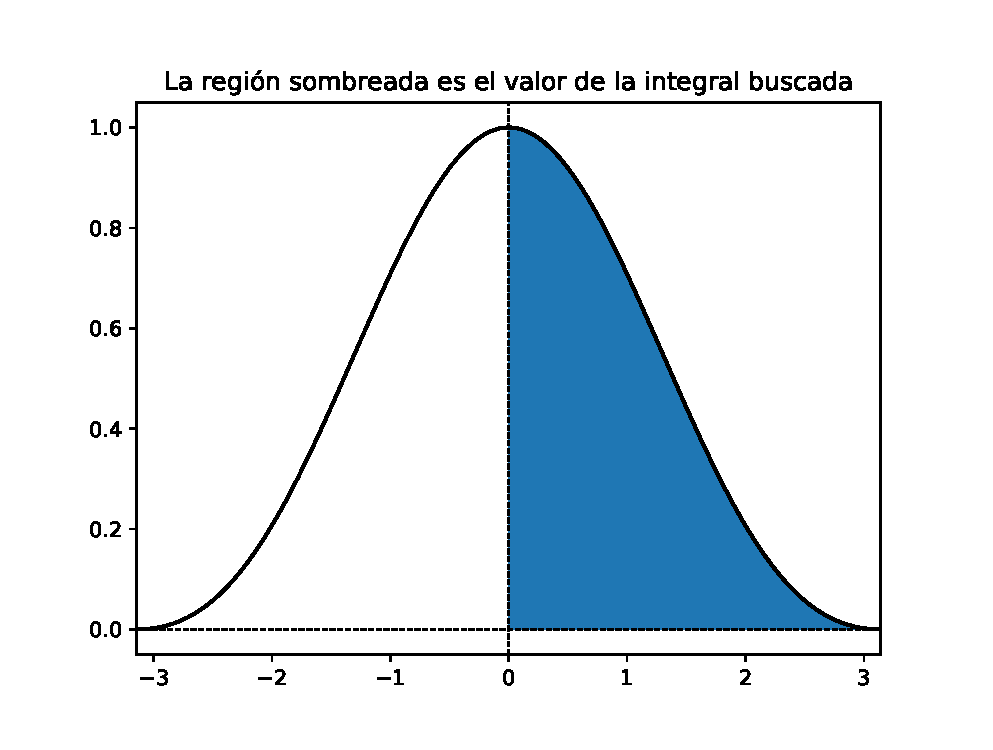
\includegraphics[scale=0.5]{Imagenes/integracion_Gauss_Legendre_01.eps}
\end{figure}
\end{frame}
\begin{frame}
\frametitle{Antes de la solución}
Presentamos la siguiente propuesta que calcula la cuadratura con $2, 3, \ldots$ nodos, hasta alcanzar la precisión deseada:
\end{frame}
\begin{frame}[allowframebreaks, fragile]
\frametitle{Solución al ejercicio 3}
\begin{lstlisting}[caption=Código para la fórmula Gauss-Legendre, style=FormattedNumber, basicstyle=\linespread{1.1}\ttfamily=\tiny, columns=fullflexible]
import numpy as np

def f(x): return (np.sin(x)/x)**2

a = 0.0
b = np.pi
Iexacta = 1.41815

for m in range(2, 12):
	I = quadGauss(f, a, b, m)
	if np.abs(Iexacta - I) < 1e-5:
		print()
		print('Numero de nodos: ', m)
		print('La integral por cuadratura vale I = {0:1.8f}'.format(I))
		break
\end{lstlisting}
\end{frame}
\begin{frame}[fragile]
\frametitle{Salida en la terminal}
El resultado que vemos en la terminal (con una rutina para calcular el error relativo) es el siguiente:
\begin{verbatim}
Número de nodos:  5
La integral por cuadratura vale 
I = 1.41815027
El error relativo es E = 1.88825e-05
\end{verbatim}
\end{frame}
\section{Paquetes y módulos con \texttt{scipy}}
\frame{\tableofcontents[currentsection, hideothersubsections]}
\subsection{Módulo disponible para integración}
\begin{frame}
\frametitle{Módulo en \texttt{python} para integración}
Una vez que hemos revisado las técnicas de integración tanto con fórmulas de Newton-Cotes como las cuadraturas Gaussianas, y hemos implementado una serie de algoritmos para evaluar las integrales, veremos la potencia de \texttt{python} al utilizar un paquete y módulo para integración numérica.
\end{frame}
\begin{frame}
\frametitle{¿Por qué comenzamos así?}
Te podrás preguntar en este momento, el por qué no iniciamos este subtema con una revisión del módulo y las funciones de integración.
\\
\bigskip
La respuesta es muy sencilla: el curso de Física Computacional, debe de ofrecerte las herramientas necesarias para resolver el tema de integración.
\end{frame}
\begin{frame}
\frametitle{¿Por qué comenzamos así?}
Una vez conocido el fundamento y el análisis del problema, entonces cuentas con los elementos necesarios para implementar en cualquier lenguaje o programa, la solución para evaluar una integral.
\end{frame}
\begin{frame}
\frametitle{¿Por qué comenzamos así?}
Nuestro curso no es propiamente un curso de programación con \texttt{python}; el haber iniciado con los módulos y funciones de integración, nos \enquote{limitan} en cuanto al análisis y fundamento del problema, no se trata de usar un conjunto de funciones debidamente (parámetros, ajustes, etc.) sino, de comprender un problema y entonces ya con ese contexto, podemos aprovechar el alcance de \texttt{python}.
\end{frame}
\subsection{Integración con (\texttt{scipy.integrate})}
\begin{frame}
\frametitle{Integración (\texttt{scipy.integrate})}
Ya hemos utilizado el paquete \funcionazul{scipy}, de ahí ocuparemos el módulo \funcionazul{scipy.integrate} que proporciona un conjunto de funciones de integración numérica:
\end{frame}
\begin{frame}
\frametitle{Integración (\texttt{scipy.integrate})}
\fontsize{12}{12}\selectfont
\begin{tabular}{l | p{8cm}}
quad 		& Integración en general. \\ \hline
dblquad 	& Integración doble en general. \\ \hline
tplquad 	& Integración triple en general. \\ \hline
fixed-quad 	& Integración de $f(x)$ usando cuadratura Gaussianas de orden $n$. \\ \hline
quadrature 	& Integra con tolerancia dada usando cuadratura Gaussiana. \\ \hline
romberg 	& Integra una función mediante la integración de Romberg.
\end{tabular}
\end{frame}
\subsection{La función \texttt{quad}}
\begin{frame}[fragile]
\frametitle{La función \texttt{quad}}
Revisaremos la sintaxis mínima de la función \funcionazul{quad}, esto quiere decir que la función contiene más argumentos, y es buena idea de que los revises en la respectiva documentación de \texttt{python}:
\end{frame}
\begin{frame}[fragile]
\frametitle{La función \texttt{quad}}
La función es:
\begin{verbatim}
quad(func, a, b)
\end{verbatim}
donde
\verb|func :|  es la función a integrar.
\\
\medskip
\verb|a : float| es el límite inferior de integración, en caso de que  $a = -\infty$, se utiliza \funcionazul{-numpy.infinity}.
\\
\medskip
\verb|b : float| es el límite superior de integración, en caso de que  $b = \infty$, se utiliza \funcionazul{numpy.infinity}.
\end{frame}
\begin{frame}[fragile]
\frametitle{Lo que devuelve la función}
La función \funcionazul{quad} devuelve (información mínima) en una tupla lo siguiente:
\\
\bigskip
\verb|y : float| \\
El valor de la integral de $a$ a $b$.
\\
\medskip
\verb|abserr : float| \\
Un estimado del error absoluto en el resultado.
\\
\bigskip
Revisa también la documentación de la función, ya que hay otros valores que se devuelven.
\end{frame}
\begin{frame}[fragile]
\frametitle{Ejemplo del uso de \texttt{integrate.quad}}
Calcula la integral
\begin{align*}
I = \int_{0}^{4} x^{2} \dd{x}
\end{align*}
Utilizando la función \funcionazul{integrate.quad} y reporta el error obtenido.
\end{frame}
\begin{frame}
\frametitle{Gráfica de la función a integrar}
Como buena medida de apoyo, graficamos la función en el intervalo de interés:
\begin{figure}[h!]
	\centering
	\includegraphics[scale=0.5]{Imagenes/integracion_modulo_quad_01.eps}
\end{figure}
\end{frame}
\begin{frame}[allowframebreaks, fragile]
\frametitle{Ejemplo del uso de \texttt{integrate.quad}}
Solución: ahorraremos código si usamos una función \textbf{lambda}. Ahora con la función \textoazul{integrate.quad}, tenemos que:
\begin{lstlisting}[caption=Código para evaluar la integral con \texttt{integrate.quad}, style=FormattedNumber, basicstyle=\linespread{1.1}\ttfamily=\tiny, columns=fullflexible]
from scipy import integrate

x_2_ = lambda x: x**2

integral, error = integrate.quad(x_2_, 0.0, 4.0)

print('La integral vale I = {0:1.10f}'.format(integral))
print('\nEl error en la evaluacion es E = {0:1.6e}'.format(error))
\end{lstlisting}
\end{frame}
\begin{frame}[fragile]
\frametitle{Resultados en la terminal}
El resultado obtenido por la función \funcionazul{integrate.quad} es
\begin{verbatim}
La integral vale I = 21.3333333333

El error en la evaluación es
E = 2.368476e-13
\end{verbatim}
\end{frame}
\subsection{La función \texttt{romberg}}
\begin{frame}
\frametitle{La función \funcionazul{romberg}}
Ahora veremos la sintaxis mínima para la función \funcionazul{romberg}, que evalúa una integral mediante la técnica de Romberg que discutimos en el subtema anterior de las fórmulas de Newton-Cotes.
\end{frame}
\begin{frame}[fragile]
\frametitle{Sintaxis para la función \funcionazul{romberg}}
\begin{verbatim}
integrate.romberg(function, a, b, 
show=False)
\end{verbatim}
\fontsize{12}{12}\selectfont
donde
\\
\verb|function|
\\
Es la función que se va a integrar.
\\
\medskip
\verb|a : float|
\\
Es el límite inferior de integración.
\\
\medskip
\verb|b : float|
\\
Es el límite superior de integración.
\\
\medskip
\verb|show = False|
\\
Imprime el arreglo triangular, el valor obtenido de la integral y el número de iteraciones que se realizaron.
\end{frame}
\begin{frame}
\frametitle{Ejemplo con la función \funcionazul{romberg}}
Evalúa la integral
\begin{align*}
I = \int_{0}^{\pi} \sin x \dd{x}
\end{align*}
con la función \funcionazul{integrate.romberg}, ajusta el parámetro para visualizar el arreglo triangular inferior, reporta el número de iteraciones que se realizaron.
\end{frame}
\begin{frame}
\frametitle{Gráfica para revisar el integrando}
Nuevamente nos apoyamos con un gráfica para revisar la función dentro de su dominio de integración:
\begin{figure}[h!]
	\centering
	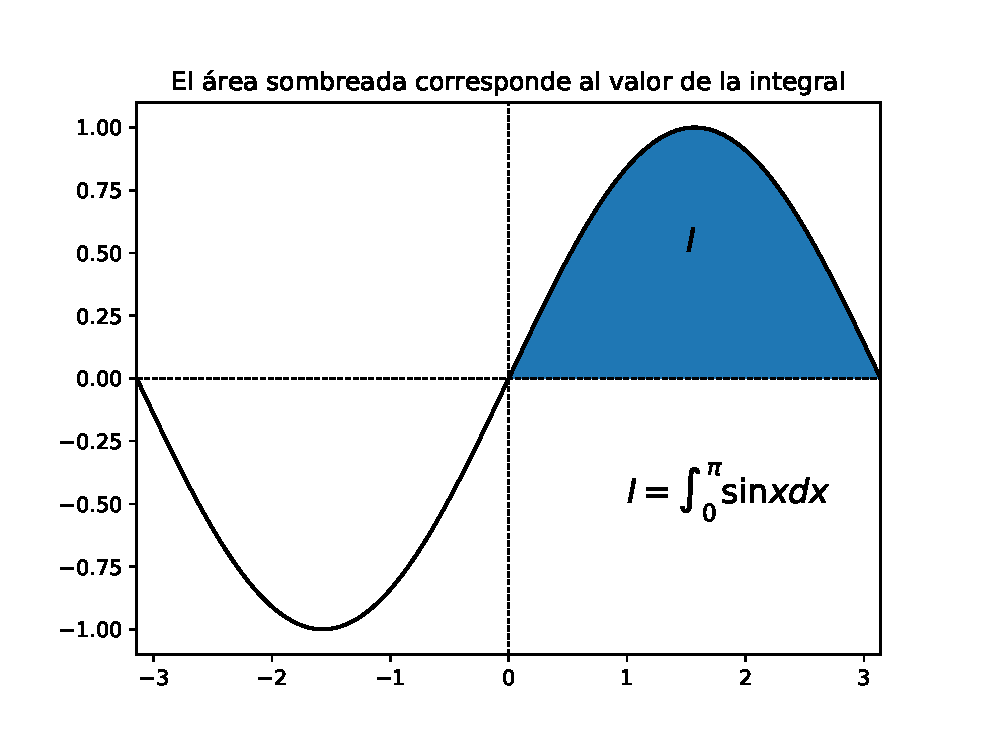
\includegraphics[scale=0.5]{Imagenes/integracion_modulo_romberg_01.eps}
\end{figure}
\end{frame}
\begin{frame}[allowframebreaks, fragile]
\frametitle{Código para el ejercicio}
\begin{lstlisting}[caption=Código para evaluar la integral con \texttt{integrate.quad}, style=FormattedNumber, basicstyle=\linespread{1.1}\ttfamily=\tiny, columns=fullflexible]
import numpy as np
from scipy import integrate

x_2_ = lambda x: np.sin(x)

integral = integrate.romberg(x_2_, 0.0, np.pi, show=1)

print(integral)	
\end{lstlisting}
\end{frame}
\begin{frame}
\frametitle{Sobre la sintaxis mínima de \funcionazul{romberg}}
Vemos que en los argumentos para resolver la integral, se proporciona la función \funcionazul{x2}, los intervalos de integración \funcionazul{a} y \funcionazul{b}, y el argumento \funcionazul{show=1}.
\\
\bigskip
\pause
Éste último nos va a desplegar el arreglo triangular inferior que se discutió también en el subtema anterior.
\end{frame}
\begin{frame}[fragile]
\frametitle{Resultado en la terminal}
\fontsize{8}{8}\selectfont
\begin{table}
\begin{tabular}{c c c c c c c c}
Steps & StepSize & Results & & & & & \\
$1$ & $3.141593$ & $0.000000$ & & & & & \\
$2$ & $1.570796$ & $1.570796$ & $2.094395$ & & & & \\
$4$ & $0.785398$ & $1.896119$ & $2.004560$ & $1.998571$ & & & \\
$8$ & $0.392699$ & $1.974232$ & $2.000269$ & $1.999983$ & $2.000006$ & & \\ 
$16$ & $0.196350$ & $1.993570$ & $2.000017$ & $2.000000$ & $2.000000$ & $2.000000$ & \\ 
$32$ & $0.098175$ & $1.998393$ & $2.000001$ & $2.000000$ & $2.000000$ & $2.000000$ & $2.000000$ \\
\end{tabular}
\end{table}
\begin{verbatim}
The final result is 2.000000000001321 after 33 function evaluations.
\end{verbatim}
\end{frame}
\subsection{Funciones para cuadraturas gaussianas}
\begin{frame}[fragile]
\frametitle{Funciones para cuadraturas gaussianas}
Dentro del tema de cuadraturas gaussianas que hemos revisado, presentamos dos funciones que evalúan la integral de una función:
\setbeamercolor{item projected}{bg=blue!70!black,fg=yellow}
\setbeamertemplate{enumerate items}[circle]
\begin{enumerate}[<+->]
\item La función \funcionazul{integrate.fixed\_quad}.
\item La función \funcionazul{integrate.quadrature}.
\end{enumerate}
\end{frame}
\begin{frame}
\frametitle{La función \funcionazul{integrate.fixed\_quad}}
La función \funcionazul{integrate.fixed\_quad} calcula la integral definida mediante una cuadratura gaussiana \emph{con $n$, un orden de integración fijo}.
\\
\bigskip
Los argumentos son:
\setbeamercolor{item projected}{bg=blue!70!black,fg=yellow}
\setbeamertemplate{enumerate items}[circle]
\begin{enumerate}[<+->]
\item La función a integrar: \textoazul{func}.
\item Los límites de integración \funcionazul{a}, \funcionazul{b}.
\item El orden \funcionazul{n} de integración.
\end{enumerate}
\end{frame}
\begin{frame}[fragile]
\frametitle{Sintaxis de \funcionazul{integrate.fixed\_quad}}
La sintaxis mínima para la función \funcionazul{integrate.fixed\_quad} es:
\begin{verbatim}
integrate.fixed_quad(func, a, b, n=5)
\end{verbatim}
\end{frame}
\begin{frame}[fragile]
\frametitle{Sintaxis de \funcionazul{integrate.fixed\_quad}}
\fontsize{12}{12}\selectfont
donde
\\
\verb|func|
\\
\medskip
Es la función a integrar.
\\
\medskip
\verb|a : float|
\\
Es el límite inferior de integración.
\\
\medskip
\verb|b : float|
\\
Es el límite superior de integración.
\\
\medskip
\verb|n : int|
\\
Es el orden de integración, en caso de no especificarlo, el valor por defecto es $n = 5$
\end{frame}
\begin{frame}[fragile]
\frametitle{Lo que devuelve la función}
La función \funcionazul{integrate.quad\_fixed} devuelve:
\\
\medskip
\verb|val : float|
\\
La aproximación a la integral.
\\
\medskip
\verb|none : None|
\\
Valor estático que devuelve \texttt{None}.
\end{frame}
\begin{frame}
\frametitle{Ejercicio con \funcionazul{fixed\_quad}}
Mediante el uso de una cuadratura gaussiana calcula la integral
\begin{align*}
I = \int_{0}^{\pi/2} \cos x \dd{x}
\end{align*}
Con $n = 4, 5$ como orden de integración, estima el error relativo considerando que la integral exacta vale $I = \sin(\pi/2) - \sin(0)$
\end{frame}
\begin{frame}
\frametitle{Gráfica de la función}
Hacemos una exploración de la función en el intervalo
\begin{figure}[h!]
	\centering
	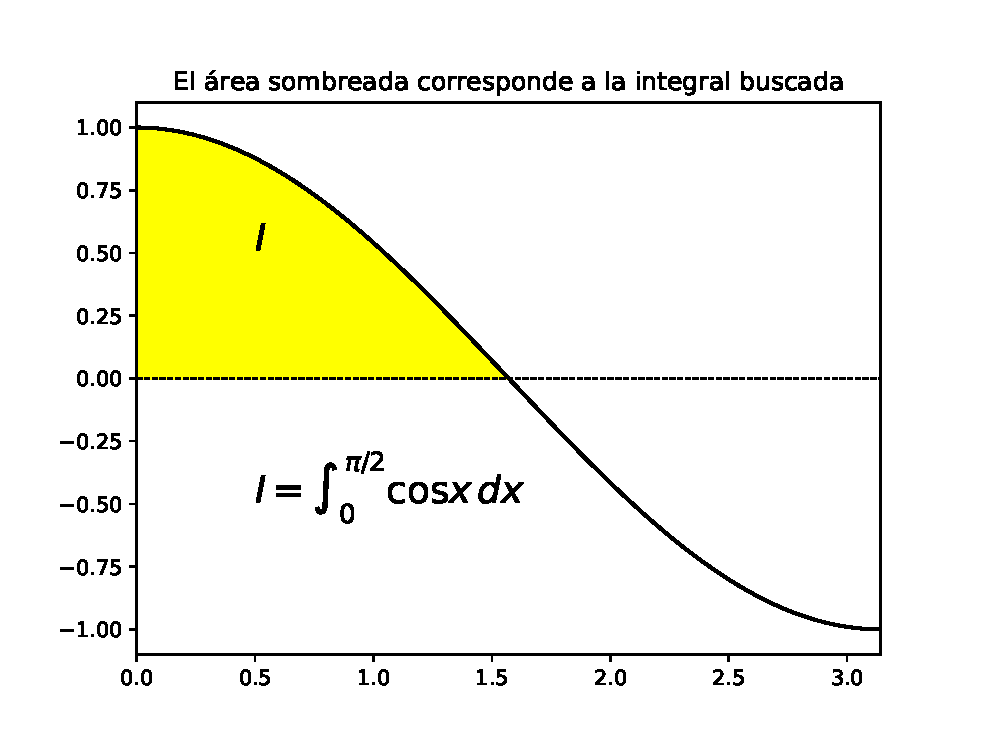
\includegraphics[scale=0.5]{Imagenes/integracion_modulo_fixed_quad_01.eps}
\end{figure}
\end{frame}
\begin{frame}[allowframebreaks, fragile]
\frametitle{Código para el ejercicio}
\begin{lstlisting}[caption=Código para resolver la integral con \texttt{integrate.fixed\_quad}, style=FormattedNumber, basicstyle=\linespread{1.1}\ttfamily=\tiny, columns=fullflexible]
import numpy as np
from scipy import integrate

f = lambda x: np.cos(x)

exacta = np.sin(np.pi/2)-np.sin(0)

print('Orden \t Integral \t \t Error')
print('--'*25)

for i in range(2):
	integral = integrate.fixed_\textunderscore_quad(f, 0.0, np.pi/2, n=i+4)
	print('{0:} \t {1:1.12f} \t {2:1.6e}'.format(i+4, integral[0]))	
\end{lstlisting}
\end{frame}
\begin{frame}
\frametitle{Comentarios al código}
Revisa que en la variable \funcionazul{integral} se toman los dos elementos que devuelve \funcionazul{integrate.fixed\_quad}: el valor de la aproximación y una etiqueta \funcionazul{None}, es por ello que en la impresión en pantalla, usamos \funcionazul{integral[0]}, que nos muestra el valor de la aproximación.
\end{frame}
\begin{frame}[fragile]
\frametitle{Resultado en la terminal}
Al ejecutar el código obtenemos lo siguiente:
\fontsize{12}{12}\selectfont
\begin{verbatim}
Orden    Integral                Error
--------------------------------------------------
4        0.999999977197          2.280288e-06
5        1.000000000040          3.956502e-09
\end{verbatim}
Por supuesto hay que incluir la respectiva rutina que evalúa el error relativo.
\end{frame}
\subsection*{La función \texttt{quadrature}}
\begin{frame}
\frametitle{La función \funcionazul{quadrature}}
La función \funcionazul{integrate.quadrature} calcula la integral definida usando una cuadratura gaussiana con una \emph{tolerancia fija}.
\\
\bigskip
A diferencia de \funcionazul{integrate.fixed\_quad}, en donde se indica el \emph{orden de integración.}
\end{frame}
\begin{frame}[fragile]
\frametitle{Sintaxis mínima para \funcionazul{integrate.quadrature}}
Para usar la función \funcionazul{integrate.quadrature} considera lo siguiente:
\begin{verbatim}
integrate.quadrature(func, a, b, 
tol=1.49e-08, maxiter=50)
\end{verbatim}
\end{frame}
\begin{frame}[fragile]
\frametitle{Argumentos de \texttt{quadrature}}
Los parámetros son:
\\
\medskip
\verb|func|
\\
Es una función de \python{} o una expresión.
\\
\medskip
\verb|a : float|
\\
Es el límite inferior de integración.
\\
\medskip
\verb|b : float|
Es el límite superior de integración.
\end{frame}
\begin{frame}[fragile]
\frametitle{Argumentos de \texttt{quadrature}}
\verb|tol : float|
\\
Es la tolerancia, este argumento es opcional. El cálculo se detiene cuando el error entre las dos últimas iteraciones es menor a \texttt{tol}.
\\
\medskip
\verb|maxiter : int|
Este argumento es opcional, representa el orden máximo para la cuadratura gaussiana.
\end{frame}
\begin{frame}[fragile]
\frametitle{Valores que devuelve la función}
La función devuelve:
\\
\medskip
\verb|val : float|
\\
Rrepresenta la aproximación a la integral.
\\
\medskip
\verb|err : float|
\\
Representa el error en las últimas dos estimaciones de la integral.
\end{frame}
\begin{frame}
\frametitle{Ejercicio con \funcionazul{quadrature}}
Evalúa la integral
\begin{align*}
\int_{0}^{\pi/2} \cos x \dd{x}
\end{align*}
mediante la cuadratura gaussiana \funcionazul{integrate.quadrature} y reporta el error obtenido en la estimación.
\end{frame}
\begin{frame}[allowframebreaks, fragile]
\frametitle{Código}
\begin{lstlisting}[caption=Código para la cuadratura gaussiana, style=FormattedNumber, basicstyle=\linespread{1.1}\ttfamily=\small, columns=fullflexible]
import numpy as np
from scipy import integrate

integral, error = integrate.quadrature(np.cos, 0.0, np.pi/2)

print('El valor de la integral es I = {0:1.16f}'.format(integral))
print('\nEl error estimado es {0:1.6e}'.format(error))
\end{lstlisting}
\end{frame}
\begin{frame}[fragile]
\frametitle{Solución en la terminal}
Lo que nos devuelve como resultado es:
\begin{verbatim}
El valor de la integral es 
I = 0.9999999999999536

El error estimado es 3.961143e-11
\end{verbatim}
\end{frame}
% \begin{frame}
% \frametitle{Ejercicios a cuenta}
% Las integrales de Fresnel
% \begin{align*}
% C(w) &= \int_{0}^{w} \cos \left( \dfrac{\pi \, u^{2}}{2} \right) \dd{u} \\
% S(w) &= \int_{0}^{w} \sin \left( \dfrac{\pi \, u^{2}}{2} \right) \dd{u}
% \end{align*}
% son un punto central en la teoría de la difracción óptica.
% \end{frame}
% \begin{frame}
% \frametitle{Ejercicio a cuenta}
% Calcula las integrales en el intervalo $w \in (-3.5, 3.5)$ con una precisión de $\varepsilon = \num{1d-6}$. Debes de resolver el problema utilizando (y justificando la elección de) la técnica de integración (código desarrollado), posteriomente usando alguna de las funciones de \python.
% \\
% \bigskip
% Grafica la curva $S(w)$ contra $C(w)$, la gráfica obtenida se le conoce como la \emph{espiral de Cornu}.
% cuerpo
% \end{frame}
\section{Ejercicios a cuenta}
\frame{\tableofcontents[currentsection, hideothersubsections]}
\subsection*{Ejercicio 1}
\begin{frame}
\frametitle{Ejercicio 1 a cuenta}
\setbeamercolor{item projected}{bg=blue!70!black,fg=yellow}
\setbeamertemplate{enumerate items}[circle]
\begin{enumerate}[<+->]
\item El período de un péndulo de longitud $L$ es
\begin{align*}
\tau = 4 \, \sqrt{\dfrac{L}{g}} \, h(\theta_0)
\end{align*}
donde $g$ es la acelaración debida a la gravedad, $\theta_{0}$ es la amplitud angular y 
\begin{align*}
h(\theta_{0}) = \int_{0}^{\pi/2} \dfrac{\dd{\theta}}{\sqrt{1 - \sin^{2} (\theta_{0}/2) \, \sin^{2} \theta}}
\end{align*}
\seti
\end{enumerate}
\end{frame}
\begin{frame}
\frametitle{Ejercicio 1 a cuenta}
Calcula $h(\ang{15})$, $h(\ang{30})$, $h(\ang{45})$, y compara esos valores con $h(0) = \pi/2$, que es la aproximación para pequeñas amplitudes.
\end{frame}
\subsection*{Ejercicio 2}
\begin{frame}
\frametitle{Ejercicio 2 a cuenta}
\setbeamercolor{item projected}{bg=blue!70!black,fg=yellow}
\setbeamertemplate{enumerate items}[circle]
\begin{enumerate}[<+->]
\conti
\item Evalúa la integral
\begin{align*}
\int_{1}^{\pi} \dfrac{\ln x}{x^{2} - 2 \, x + 2} \dd{x}
\end{align*}
mediante la cuadratura de Gauss-Legendre. Usando: a) dos nodos, b) cuatro nodos.
\seti
\end{enumerate}
\end{frame}
\subsection*{Ejercicio 3}
\begin{frame}
\frametitle{Ejercicio 3 a cuenta}
\setbeamercolor{item projected}{bg=blue!70!black,fg=yellow}
\setbeamertemplate{enumerate items}[circle]
\begin{enumerate}[<+->]
\conti
\item Con la cuadratura Gauss-Laguerre evalúa la integral
\begin{align*}
\int_{0}^{\infty} (1 - x^{2})^{3} \, e^{-x} \dd{x}
\end{align*}
\seti
\end{enumerate}
\end{frame}
\subsection*{Ejercicio 4}
\begin{frame}
\frametitle{Ejercicio 4 a cuenta}
\setbeamercolor{item projected}{bg=blue!70!black,fg=yellow}
\setbeamertemplate{enumerate items}[circle]
\begin{enumerate}[<+->]
\conti
\item Usa la cuadratura Gauss-Chebychev con seis nodos para evaluar la integral
\begin{align*}
\int_{0}^{\pi/2} \dfrac{\dd{x}}{\sqrt{\sin x}} \dd{x}
\end{align*}
Calcula el error relativo considerando que el valor exacto es $I=2.62206$. De manera directa no será posible usar la cuadratura, pero si haces el cambio de variable $\sin x = t^{2}$, ya será posible.
\end{enumerate}
\end{frame}
\subsection*{Observaciones a los ejercicios}
\begin{frame}
\frametitle{Observaciones de los ejercicios}
En cada uno de los ejercicios se deberá de resolver mediante el código que se implementó en \python, así como utilizando el paquete y librería \funcionazul{scipy.integrate}.
\end{frame}	
\end{document}